\documentclass[10pt]{article} % 5p gir 2 kolonner pr side. 1p gir 1 kolonne pr side.


% Defines fonts and language settnings
%%%%%%%%%%%%%%%%%%%%%%%%%%%%%%%%%%%%%%%%%%%%%%%%%%%%%%%%%%%%%%%
\usepackage[T1]{fontenc}
\usepackage{lmodern}
\usepackage[utf8]{inputenc}
\usepackage[english]{babel} % Tilpasning til norsk.

% Defines prettier tables and quotes
%%%%%%%%%%%%%%%%%%%%%%%%%%%%%%%%%%%%%%%%%%%%%%%%%%%%%%%%%%%%%%%
\usepackage{booktabs}
\usepackage{csquotes}


% Mathematics
%%%%%%%%%%%%%%%%%%%%%%%%%%%%%%%%%%%%%%%%%%%%%%%%%%%%%%%%%%%%%%%
\usepackage{mathtools, amsfonts, amssymb} %amsmath is loaded by mathtools

\usepackage{amsthm} %Theorems
    \newtheorem{lemma}{Lemma}
    \newtheorem{proposition}{Proposition}
    \newtheorem{definition}{Definition}

    

\usepackage{subcaption} \usepackage{caption}

% Properly defines units and spacing in numbers, use \num and \IS{size}{unit}
%%%%%%%%%%%%%%%%%%%%%%%%%%%%%%%%%%%%%%%%%%%%%%%%%%%%%%%%%%%%%%%
\usepackage{siunitx} 
    \sisetup{exponent-product = \cdot}      % Dot as multiplication symbol 
    \sisetup{output-decimal-marker  =  {,}} % Comma as decimal marker
    \sisetup{separate-uncertainty = true}   % Pluss-minus symbol for uncertanty.
    \sisetup{table-number-alignment = right ,
             table-format=2.3,
             per-mode=symbol}
    \sisetup{math-micro=\text{µ},text-micro=µ}
\usepackage{textcomp}


% Defines the ProjectEuler environment and required packages
%%%%%%%%%%%%%%%%%%%%%%%%%%%%%%%%%%%%%%%%%%%%%%%%%%%%%%%%%%%%%%%
\usepackage[dvpipsnames*,svgnames]{xcolor}
\usepackage{tikz}
\usetikzlibrary{trees}
\usepackage[framemethod=TikZ]{mdframed}

\newenvironment{ProjectEuler}[2][]{%

\setcounter{section}{#2}

\addcontentsline{toc}{section}{Project Euler~#2:~#1}
\ifstrempty{#1}%
{\mdfsetup{%
frametitle={%
\tikz[baseline = (current bounding box.east), outer sep = 0pt]
\node[anchor = east, rectangle, fill = blue!20]
{\strut Project Euler~#2};}}
}%
{\mdfsetup{%
frametitle={%
\tikz[baseline = (current bounding box.east),outer sep = 0pt]
\node[anchor = east, rectangle, fill = blue!20]
{\strut \hypersetup{urlcolor = {}}\href{https://projecteuler.net/problem=#2}{Project Euler~#2:~#1}\hypersetup{urlcolor = cyan}};}}%
}%
\mdfsetup{innertopmargin=10pt, linecolor=blue!20,%
linewidth = 2pt, topline = true,%
frametitleaboveskip=\dimexpr-\ht\strutbox\relax
}
\begin{mdframed}[]\relax%
\label{PE-#2}}{\end{mdframed}}


% Centeres figures automagically
%
%%%%%%%%%%%%%%%%%%%%%%%%%%%%%%%%%%%%%%%%%%%%%%%%%%%%%%%%%%%%%%%
\makeatletter
\g@addto@macro\@floatboxreset\centering
\makeatother


% Defines the style for the codeblocks
%
%%%%%%%%%%%%%%%%%%%%%%%%%%%%%%%%%%%%%%%%%%%%%%%%%%%%%%%%%%%%%%%
\usepackage{listings, chngcntr}
\usepackage{geometry}
\geometry{left=1.0in,right=1.0in,top=1.0in,bottom=1.0in }

\lstset{ frame=top,frame=bottom,
  stepnumber=1, % the step between two line-numbers. If it is 1 each line will be numbered
  numbersep=10pt, % how far the line-numbers are from the code
  tabsize=2, % tab size in blank spaces
  extendedchars=true, %
  breaklines=true, % sets automatic line breaking
  captionpos=t, % sets the caption-position to top
  mathescape=true,
  literate=
         {=}{$\leftarrow{}$}{1}
         {+=}{${}\uparrow{}$}{2}
         {==}{$={}$}{2}
         {||}{OR}{2},
  showspaces=false, % Leerzeichen anzeigen ?
  showtabs=false, % Tabs anzeigen ?
  xleftmargin=17pt, framexleftmargin=17pt, framexrightmargin=17pt,
  framexbottommargin=5pt,
  framextopmargin=5pt,
  showstringspaces=false % Leerzeichen in Strings anzeigen ?
} \lstMakeShortInline[columns=fixed]|

\DeclareCaptionFormat{listing}{\rule{\dimexpr\textwidth+17pt\relax}{0.4pt}\par\vskip1pt#1#2#3}
\captionsetup[lstlisting]{format=listing,singlelinecheck=false, margin=0pt,
  font={sf},labelsep=space,labelfont=bf}

\renewcommand\lstlistingname{Algorithm}

%%
%% Julia definition (c) 2014 Jubobs
%%
%%%%%%%%%%%%%%%%%%%%%%%%%%%%%%%%%%%%%%%%%%%%%%%%%%%%%%%%%%%%%%%
\lstdefinelanguage{Julia}%
  {morekeywords={abstract,break,case,catch,const,continue,do,else,elseif,%
      end,export,false,for,function,immutable,import,importall,if,in,%
      macro,module,otherwise,quote,return,switch,true,try,type,typealias,%
      using,while},%
   sensitive=true,%
   alsoother={$},%
   morecomment=[l]\#,%
   morecomment=[n]{\#=}{=\#},%
   morestring=[s]{"}{"},%
   morestring=[m]{'}{'},%
}[keywords,comments,strings]%

\lstset{%
    language         = Julia,
    keywordstyle     = \bfseries,
    stringstyle      = \color{magenta},
    commentstyle     = \color{ForestGreen},
    showstringspaces = false,
}
% Hyper references
%
%%%%%%%%%%%%%%%%%%%%%%%%%%%%%%%%%%%%%%%%%%%%%%%%%%%%%%%%%%%%%%%%%%%%%%%%%

\usepackage{hyperref}
\hypersetup{colorlinks=true,
            pdfmenubar=false,
            pdfstartview={FitH},
            linktoc = all,
            urlcolor = purple,
            citecolor = black,
            linkcolor = {}}

\usepackage[nameinlink]{cleveref}


%%%%%%%%%%%%%%%%%%%%%%%%%%%%%%%%%%%%%%%%%%%%%%%%%%%%%%%%%%%%%%%%%%%%%%%%%

% Bibliography

%%%%%%%%%%%%%%%%%%%%%%%%%%%%%%%%%%%%%%%%%%%%%%%%%%%%%%%%%%%%%%%%%%%%%%%%%

\usepackage[numbers]{natbib}
\usepackage{chapterbib}

%%%%%%%%%%%%%%%%%%%%%%%%%%%%%%%%%%%%%%%%%%%%%%%%%%%%%%%%%%%%%%%%%%%%%%%%%

\usepackage{multicol}

%Defines the linkcolor 
\newcommand{\link}{NavyBlue}

\usepackage[nameinlink]{cleveref}

\creflabelformat{equation}{#2(\textcolor{\link}{#1})#3}
\creflabelformat{table}{#2\textcolor{\link}{#1}#3}
\creflabelformat{figure}{\!#2\textcolor{\link}{#1}#3}

\title{Project Euler \\ - Prematurely optimized and Overengineered }
\author{Øistein Søvik}

% \includeonly{Problems/PE-014}

\begin{document}
\counterwithin{lstlisting}{section}

\begin{titlepage}
\begin{center}
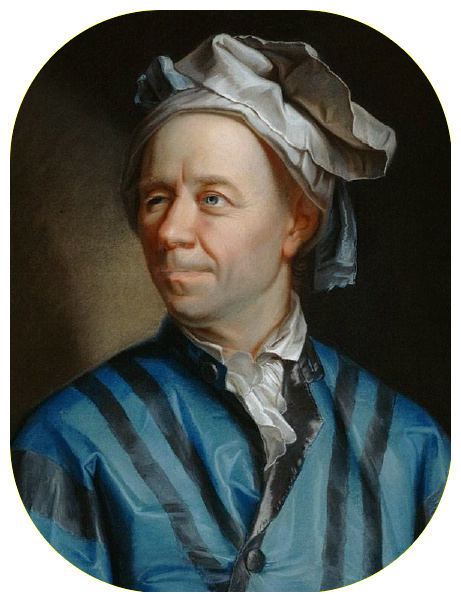
\includegraphics[width=0.20\textwidth]{../Images/portrait.png}~\\[1cm]

\textsc{\LARGE Project Euler}\\[1.5cm]

% \textsc{\Large TDT4136 - Introduction to Artificial Intelligence}\\[0.5cm]

% Title
\rule{\linewidth}{0.5mm} \\[0.4cm]
{ \huge \bfseries Prematurely optimized \& overengineered solutions}\\[0.5cm]
{\large \textit{Oistein Sovik}}\\[0.2cm]
\rule{\linewidth}{0.5mm} \\[1.5cm]



\vfill

% Bottom of the page
{\large \today}
\end{center}
\end{titlepage}

%%% Local Variables:
%%% TeX-master: "ProjectEuler"
%%% End:

\tableofcontents

\section*{Preface}

This project has been ressurected twice, and thus this version might be thought
of as Project Euler 1.2. One main difference is that the codebase is now avaible
on Github:
%
\begin{center}
  \url{https://github.com/Oisov/Project-Euler}.
\end{center}
%
Another major change is the addition of several other programming languages,
with the most prominent being \textbf{Julia}. The code in these notes are now
written in Julia as it closely resembles psudocode, with just a few minor
changes.
%
\begin{enumerate}
    \item The logical expressions $\|\|, \&\&, !$ has been replaced with
          \textsc{OR}, \textsc{AND}, \textsc{NOT}
    \item Variable declaration is changed from $=$ to $\rightarrow$
    \item Variable comparison $==$ is changed to $=$
    \item The $+=$ syntax used to represent increasing a variable is replaced
    with $\uparrow$
\end{enumerate}
%
What has \emph{not} changed is the purpose of this document. The goal is still
to present well written, clever and interesting solutons to Project Euler.

I have seen too many hastily written solutions to these problems. While the
solutions work, they are not written in a clear matter, single letter
variablenames and no function declarations. Code like this is incredibly hard to
read for someone who has not produced the mess, and even for the author the code
can be incomprehensible after just a few weeks.

While I can not hope to remedy every badly written code with these notes,
hopefully someone who reads these notes, or browses the github repo finds some
inspiration. 

\begin{ProjectEuler}[Even Fibonacci numbers]{1}
  Each new term in the Fibonacci sequence is generated by adding the previous
  two terms. By starting with 1 and 2, the first 10 terms will be:
  %
  \begin{align*}
    1, 2, 3, 5, 8, 13, 21, 34, 55, 89, ...
  \end{align*}
  %
  By considering the terms in the Fibonacci sequence whose values do not exceed
  four million, find the sum of the even-valued terms.
\end{ProjectEuler}

\begin{lstlisting}[language=Julia, caption=Naive recursive solution]
    def fib(n):
        if n in [0, 1]:
            return n
        else:
            return fib(n-1) + fib(n-2)
            
    function PE_002_recursive_naive(limit)
        n = 0 
        total = 0
        while fib(n) < limit
            n += 1
            if fib(n) % 2 == 0:
                total += fib(n)
	      return total
\end{lstlisting}

%%% Local Variables:
%%% TeX-master: "../ProjectEuler"
%%% End:




\begin{ProjectEuler}[Lattice paths]{15}
  Starting in the top left corner of a 2×2 grid, and only being able to move to
  the right and down, there are exactly 6 routes to the bottom right corner.
  %
  \begin{center}
    
\includegraphics[scale=0.5]{../Images/PE_015.png}
  \end{center}
  %
  How many such routes are there through a $20\times20$ grid?
\end{ProjectEuler}

\subsection{Recursive solution}

\lstinputlisting[language=Julia, 
                 caption=Recursive route-counting function,
                 ]{../Problems/PE_015/Julia/PE_015_recursive.jl}

To speed up this code we could have defined
\lstinline|path_sum[(m,n)]=path_sum[(n,m)]| and as we know that there are only
one way to reach each of the points on the first column and first row. However,
while this halves the number of function calls this is not where the bottleneck
lies. Most of the time is spent looking up dictionary values. 

\newpage

\subsection{Iterative solution}

While the memoized recursion solves the problem, it is not only slow, but
requires more memory, and some languages have trouble with deeply-nested
recursive calls.

If we could translate our recursion into and \emph{iterative} solution using
bottom-up programming technique called \emph{dynamic programming} we would solve
most of the concerns raised above. 
\lstinputlisting[language=Julia, 
                 caption=Recursive route-counting function,
                 ]{../Problems/PE_015/Julia/PE_015_iterative.jl}

                 \subsection{Combinatorial solution}
                 
\lstinputlisting[language=Julia, 
                 caption=Recursive route-counting function,
                 ]{../Problems/PE_015/Julia/PE_015.jl}
%%% Local Variables:
%%% TeX-master: "../ProjectEuler"
%%% End:

\end{document}